\documentclass{article}
\usepackage{hyperref}
\usepackage{graphicx}
\graphicspath{ {foto_translate/} }
\usepackage{anyfontsize}


\title{GridWorld : Part 2}
\author{abidghozi}


\begin{document}
	\newpage
	
	\section*{GridWorld : Part 2}
	Part ke 2 dari studi kasus pada GridWorld akan menggunakan beberapa fitur yang belum pernah kita lihat sebelumnya, maka kamu akan mendapatkan contoh lebih banyak dibandingkan dengan penjelasan yang lebih detailnya, sebegai pengingat, kamu dapat mencari kumpulan dokumentasi untuk class yang ada pada GridWorld di 
	\url{http://www.greenteapress.com/thinkapjava/javadoc/gridworld/}
	\\
	
	Ketika kamu menginstall GridWorld, kamu akan mendapatkan folder yang bernama ‘projects/boxBug’, yang dimana akan berisi BoxBug.java, BoxBugRunner.java dan BoxBug.gif.
	\\
	
	Salin file tersebut ke dalam folder dimana kamu bekerja dan import file tersebut ke dalam lokasi file kerja kalian(development environment). Disini terdapat beberapa langkah yang mungkin dapat membantu \url{http://www.collegeboard.com/prod_downloads/student/
	testing/ap/compsci_a/ap07_gridworld_installation_guide.pdf}
	\\
	
	Ini adalah code dari BoxBugRunner.java :
	\\
	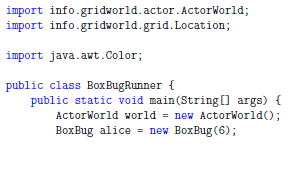
\includegraphics{A1}
	\\
	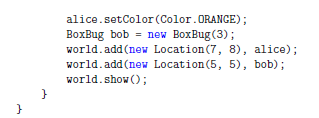
\includegraphics{A2}
	\\
	
	Semua yang terdapat pada code tersebut seharusnya terlihat familiar, dengan pengecualian untuk lokasi yang dimana ini merupakan bagian dari GridWorld dan mirip seperti java.awt.Point
	\newpage
	
	BoxBug.java memilki class yang mendifinisikan bagian dari BoxBug
	\\
	\\
	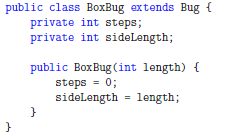
\includegraphics{B1}
	\\
	Baris pertama pada code tersebut menjelaskan bahwa class ini merupakan bagian dari Bug, yang berarti BoxBug merupakan salah satu jenis Bug.
	\\
	
	Lalu pada 2 baris berikutnya merupakan instance variables. Setiap Bug memiliki variables yang bernama sideLength, yang dapat diartikan sebagai ukuran box yang digambarkan, dan langkahnya, yang akan memantau berapa banyak langkah yang telah Bug lakukan.
	\\
	
	Baris berikutnya menjelaskan tentang Constructor yaitu metodee special yang berguna untuk membuat nilai awal pada instance variables. Ketika kamu membuat Bug dengan menggunakan new, java akan menggunakan constructor ini.
	\\
	
	Parameter untuk constructor ini adalah sideLength.
	\\
	
	Kelakuan dari Bug di kendalikan oleh metodee bernama act. Dibawah ini adalah metodee act untu BoxBug : 
	\\
	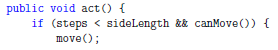
\includegraphics{C1}
	\\
	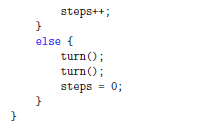
\includegraphics{C2}
	\\
	
	Jika BoxBug dapat bergerak, dan tidak mengambil angka yang dibutuhkan untuk setiap steps maka ia akan bergerak dan menambahkan steps setiap kali ia bergerak.
	\\
	
	Jika ia berhenti atau sudah berada pada kondisi akhir, maka ia berubah 90 derajat ke kanan dan kembari mereset steps ke 0.
	\\
	
	Jalankan programnya dan lihat apa yang dilakukan. Apakah kamu mendapatkan langkah yang seperti kamu inginkan?
	\\
	
	\section*{10.1 Termites}
	Saya menulis class yang bernama Termite yang merupakan bagian dari Bug dan menambahkan kemampuan untuk berinteraksi dengan flowers. Untuk menjalankannya, download file tersebut dan import ke dalam lokasi kamu membuat program tersebut : 
	\\
	
	\url{http://thinkapjava.com/code/Termite.java}
	\url{http://thinkapjava.com/code/Termite.gif}
	\url{http://thinkapjava.com/code/TermiteRunner.java}
	\url{http://thinkapjava.com/code/EternalFlower.java}
	\\
	
	Dikarenakan Termite merupakan bagian dari Bug, semua metode yang ada di Bug juga dapat dilakukan di dalam Termites. Tetapi Termites memiliki metode tambahan yang tidak dimiliki oleh Bug.
	\newpage
	
	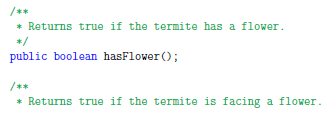
\includegraphics{D1}
	\\
	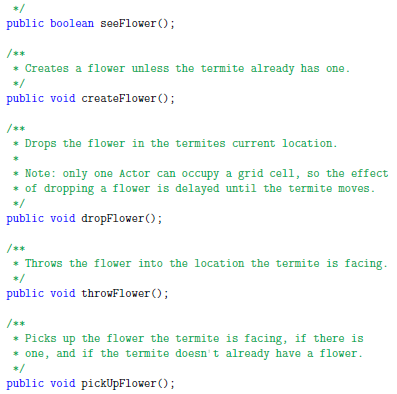
\includegraphics{D2}
	\\
	
	{\small Penjelasan Komentar}\\
	{\footnotesize comment 1 : Kembalikan True jika termite memiliki flower}\\
	{\footnotesize comment 2 : Kembalikan True jika termite bertemu dengan flower}\\
	{\footnotesize comment 3 : Buat flower kecuali termite sudah memiliki satu}\\
	{\footnotesize comment 4 : Jatuhkan flower di lokasi termites saat itu}\\
	{\footnotesize comment 5 : Lempar flower ke arah pandang termite}\\
	{\footnotesize comment 6 : Ambil flower dimana termite melihatnya, jika terdapat satu dan jika termite belum memiliki flower}\\
	\newpage
	
	Untuk beberapa metodee Bug menyediakan satu ketentuan dan Termite menyediakan yang lain dalam suatu kasus, metode yang dimiliki Termite akan mengesampingkan metode Bug.
	\\
	
	Untuk contohnya, ‘Bug.canMove’ mengembalikan True jika disana terdapat flower di lokasi berikutnya, maka Bugs juga dapat menginjak flowers. Termite.canMove ajan mengembalikan False jika disana terdapat object di lokasi beriktunya, maka Termite dapat melakukan hal yang berbeda dari Bug.
	\\
	
	Dalam contoh lain, Termites memiliki versi dari langkah yang dia ambil menggunakan integer sebagai parameter. Yang akhirnya Termites memiliki ‘randomTurn’. Yaitu dapat berbalik 45 derajat ke kiri atau kanan secara acak.
	\\
	
	Ini code dari TermiteRunner.java : 
	\\
	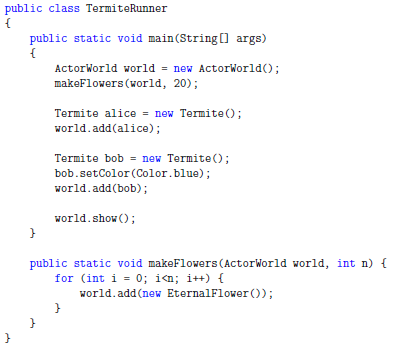
\includegraphics{E1}
	\\
	
	Semua yang ada di dalam code tersebut mungkin terlihat tidak asing. TermiteRunner membuat ActorWorld dengan 20 EternalFlowers dan 2 Termites.
	\\
	
	EternalFlower adalah bunga yang dapat mengesampingkan act jadi flowers tidak terlihat menggelap.
	\\
	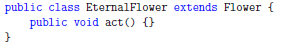
\includegraphics{F1}
	\\
	
	Jika kamu menjalankan TermiteRunner.java kamu akan melihat 2 termites berjalan secara acak diantara flowers.
	\\
	
	MyTermite.java mendemonstrasikan metode yang berinteraksi dengan flowers. Ini salah definisi dari class tersebut : 
	\\
	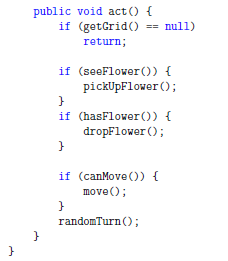
\includegraphics{G1}
	\\
	
	MyTermite merupakan class bagian dari Termite dan mengesampingkan act. If MyTermite melihat flower, ia akan mengambilnya. Jika ia memiliki flower, maka jatuhkan bunganya.
	\\
	
	\section*{10.2 Langton's Termite}
	Langton’s Ant adalah model sederhana dari bagaimana ant bertindak yang menampilkan tindakan yang sangat complex. The Ant tinggal di dalam grid seperti GridWorld dimana setiap cell dalah putih atau hitam. The Ant bergerak menurut perintah tersebut : 
	\\
	
	\begin{itemize}
		\item Jika The Ant ada di cell yang berwarna putih, maka ia akan merubah arah ke kanan, membuat cell tersebut menjadi berwarna hitam dan maja kedepan.
		\item Jika The Antada di cell yang berwarna hitam, maka ia akan merubah arah ke kiri, dan membuat cell tersebut menjadi berwarna putih dan maju kedepan.
	\end{itemize}
	\newpage
	
	Dikarenankan peraturan tersebut sangatlah sederhana, kamu mungkin mengira bahwa The Ant akan melakukan sesuatu yang sederhana seperti membuat kotak atau mengulang pola sederhana yang sama. Tetapi dimulai dari semua cell yang berwarna putih, The Ant membuat lebih dari 10,000 langkah yang acak sebelum berubah ke perulangan yang sama sebanyak 104 langkah.
	\\
	
	Kamu dapat membaca lebih banyak dari Langton’s Ant di \\
	\url{http://en.wikipedia.org/wiki/Langtin_ant}
	\\
	
	Ini tidak mudah untuk mengimplementasikan Langton’s Ant di dalam GridWorld karena kita dapat merubah warna dari cells. Sebagai alternatif kita dapat menggunakan Flowers untuk menandakan cells, tetapi kita tetap tidak dapat membuat Ant dan Flower berada di dalam cell yang sama maka dari itu kita tidak dapat mengimplementasikan aturan The Ant secara tepat.
	\\
	
	Sebagai gantiya kita akan membuat apa yang disebut LangtonTermite, dimana menggunakan ‘seeFlower’ untuk mengecek apakah terdapat Flower di cell berikutnya, ‘pickUpFlower’ untuk mengambil dan ‘throwFlower’ untuk menaruh Flower di cell berikutnya. Kamu mungkin ingin membaca code dari metode tersebut untuk meyakinkan bahwa kamu mengetahui apa yang mereka lakukan.
	\\
	
	\section*{10.3 Latihan}
	\subsection*{Latihan 10.1}
	Sekarang kamu sudah cukup memahami untuk mengerjakan latihan yang ada pada pedoman siswa, Part 2. Kerjakan latihan tersebut, dan kembali untuk mendapatkan hal yang lebih.
	\\
		
	\subsection*{Latihan 10.2}
	Tujuan dari latihan ini adalah untuk mengetahui tingkah laku dari Termites yang berinteraksi dengan Flowers.
	\\
	
	Ubah TermiteRunner.java untuk membuat MyTermites untuk menggantikan Termites. Lalu jalankan lagi. MyTermites harus dapat bergerak secara acak, dan membawa bunga. Total dari bunga harus sama(termasuk yang dapat MyTermites bawa)
	\newpage
	
	Di dalam ‘Termites, Turtles and Traffic Jams’, Mitchell Resnick menjelaskan tindakan sederhana yang dilakukan oleh termite sebagai berikut : 
	
	\begin{itemize}
		\item Jika dia melihat flower, maka ambil. Kecuali dia sudah memiliki bunga tersebut dalam hal tersebut maka jatuhkan yang kamu punya.
		\item Maju kedepan jika dia bisa.
		\item Belok kiri atau kanan secara acak.
	\end{itemize}
	
	Ubah MyTermite.java untuk mengimplementasikan model tersebut. Menurut kamu efek apa yang akan terjadi pada tingkah laku dari MyTermites?
	\\
	
	Coba lagi, lalu selanjutya, total flower yang ada tidak berubah namun secara beberapa waktu the flowers akan muncul dalam tumpukan yang kecil, terkadang hanya satu.
	\\
	
	Tingkah laku ini ada di dalam ‘an emergent property’, yang dapat kamu baca di \url{http://en.wikipedia.org/wiki/Emergence}. MyTermites mengikuti peraturan sederhana dengan hanya menggunakan informasi berskala kecil, tetapi dengan hasil organisasi dengan skala yang besar.

	Bereksperimenlah dengan peraturan yang berbeda dan lihat efek apa yang akan terjadi pada sistem tersebut. Perubahan kecil dapat menghasilkan hasil yang tidak terduga.

	\subsection*{Latihan 10.3}
	\begin{enumerate}
		\item Buat salinan dari Termite.java dengan nama LangtinTermite dan salinan dari TermiteRunner.java dengan nama LangtonRunner.java ubah file tersebut sehingga classnya sama dengan file dan juga LangtinRunner membuat LangtonTermite.
		\item Jika kamu membuat file bernama LangtonTermite.gif, GridWorld menggunakan itu untuk menampilkan Termite kamu, kamu dapat mengunduh gambar-gambar serangga yang bagus dari \url{http://www.cksinfo.com/animals/insects/realisticdrawings/index.html}. Untuk mengubah file tersebut ke dalam format GIF, kamu dapat menggunakan aplikasi seperti ImageMagick.
		\item Ubah act untuk mengimplementasikan peraturan yang mirip dengan Lanton’s Ant. Coba bereksperimantasilah dengan berbagai macam peraturan dan dengan belokan 45 dan 90 derajat. Cari aturan yang paling memiliki banyak langkah sebelum Termite memulai pengulangan langkah.
		\item Untuk membuat Termite ruangan yang cukup besar, kamu dapat membuat gridnya lebih besar atau ubah ke UnboudedGrid.
		\item Buat lebih dari satu LangtonTermite dan lihat bagaimana mereka berinteraksi.
	\end{enumerate}
	
	
\end{document}